% Giving the thesis a purpose (not how, but why)
%   Mention problems in industry practice (mention software product lines)
%   Say what software product lines are for, not technicalities, why they exist
%   Talk about why planning is difficult, when the project size is increasing
%   -> Changing the plan is even more difficult, and there is a lack of automated tools for checking that the changes don't break anything
%   Drawing a picture of the domain and the problem
%   My thesis is addressing these challenges by looking at these research questions or goals
% Last part of introduction: research questions/goals (base structure of thesis on this) - 3 is a good number
% They are general. What, how, (never why)
% In this thesis, I will address these questions through these activities ...(will not tackle everything, so make the purpose clear)
% Start broader, chunk down to more detail
% Can take the goals up again in the following sections (mention the research questions when tackling them)
% How the sensor should read my master's thesis. How will she know what my contribution is, where it comes in. "In chapter 2 I will give the background, limited to the scope of my thesis". Make it clear that I'm not trying to cover everything, and give the logic/structure of the thesis.

% Storyline: SPLs -> planning -> existing solution (LTEP) -> problem with that solution -> goal

% High-level introduction to software product lines

% Can talk about static analysis in terms of related work or background.
% -> Semantic-based analysis
% -> Forward analysis and scope (live variable analysis etc)
% - Bring up research questions after this

% Reference previous work clearly, talk about how my work builds upon it.
\chapter{Introduction}
\label{cha:introduction}

A software product line (SPL) capitalizes on the similarity and variability of closely related software products~\cite{book:introduction-to-spl}. The similarities and variability are captured by features, which are customer-visible characteristics of a system~\cite{book:introduction-to-spl}. Each product in the product line (called a \textit{variant}) comprises a selection of these features, resulting in a flexible and customizable set of variants available to customers. To model an SPL it is common to use a feature model, a tree-like structure with nodes representing features. From this model, a variant can be derived by selecting features. The feature model's structure creates restrictions for which variants are allowed, while they also make it possible to model all possible variants at once~\cite{art:feature-models-grammars-and-propositional-formulas}.

SPLs grow large as they are more profitable the more variants they originate~\cite{book:introduction-to-spl}, % page 10 (34 absolute)
and evolve over time as requirements change~\cite{art:context-aware-reconfiguration-in-evolving-software-product-lines, art:darwinspl-an-integrated-tool-suite-for-modeling-evolving-context-aware-software-product-lines}. Complex projects require planning~\cite{art:evofm-feature-driven-planning-of-product-line-evolution}. Intuitively, this means describing how the feature model should look at a future point in time. For instance, new technology may emerge that the manager wishes to incorporate in the product line, but which takes a year to implement. One can then plan how the feature model will look at that point, as well as at some earlier stages where the technology is partly included. However, as requirements change, plans must adapt, and it may be necessary to change an existing plan, for instance by removing or adding features. These retroactive changes can affect later parts of the plan, causing \emph{paradoxes} that make the plan impossible to realise~\cite{art:anomaly-detection-and-explanation-in-context-aware-software-product-lines}. 

\begin{figure}
   \begin{centering}
      \begin{minipage}[t]{0.42\textwidth}
         \vspace{0pt}
         \small
         \begin{center}
            Original plan
         \end{center}
         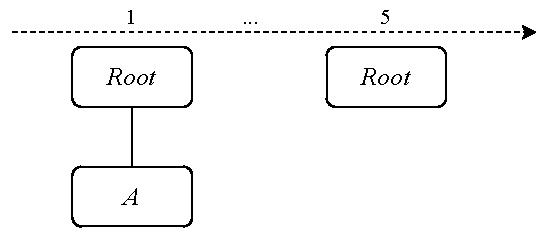
\includegraphics[width=\textwidth]{SimpleParadox1}
      \end{minipage}\hfill
      \begin{minipage}[t]{0.56\textwidth}
         \vspace{0pt}
         \small
          \begin{center}
             Modified plan
          \end{center} 
         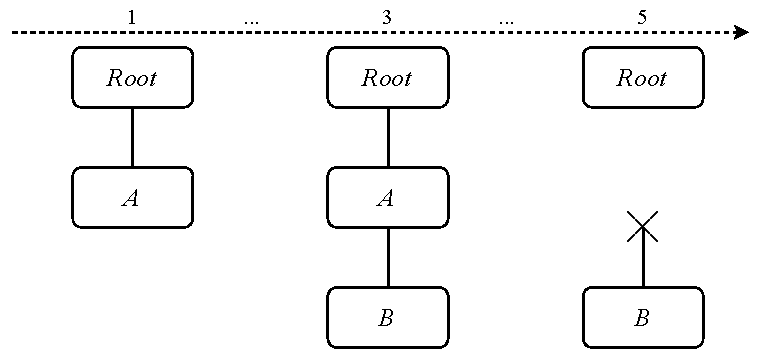
\includegraphics[width=\textwidth]{SimpleParadox2}
      \end{minipage}
   \end{centering}
   \caption{Simple paradox}
   \label{ex:simple-paradox}
\end{figure}

A simple example of a paradox can be seen in Figure~\vref{ex:simple-paradox}. Here, a feature model is illustrated as a normal tree for simplicity. In the original plan, a node $A$ exists in time $1$ and is removed at time $5$. We modify the plan by adding a child node $B$ to $A$ at time $3$. This change causes a paradox in time $5$, since node $B$ is left without a parent node. In this case, it would be simple to detect this paradox by hand, but given a plan with hundreds of nodes and points in time, paradoxes may be harder to locate.  Thus, there is a need for tooling that supports safe retroactive change to feature model evolution plans. 

Notice also the difference between \emph{feature model change}, i.e. planning to remove $A$ at time $5$, and \emph{plan change}, i.e. modifying the original plan by introducing $B$ at time 3. A plan may contain many changes to a feature model, but an evolution process will change the plans themselves. In this thesis we focus on plan changes.

\section{The LTEP Project}
\label{sec:the-ltep-project}
% Se prosjektbeskrivelsen, kanskje i søknaden til NFR og DAAD. (project proposal)
This thesis is part of the LTEP research project, which was initiated in 2019 to address the lack of methodology and tooling for planning the long-term evolution of software product lines. It is a collaboration between the University of Oslo and the German university Technische Universität Braunschweig. The overarching goal of the project is to create methodology for the long-term evolution planning of SPLs, and we have published a paper~\cite{art:consistency-preserving-evolution-planning} giving methods for verifying soundness of \emph{feature model evolution plans} (FMEPs). 

This method lets us detect paradoxes in a feature model evolution plan, and has been integrated into the SPL planning tool DarwinSPL\footnote{\url{https://gitlab.com/DarwinSPL/DarwinSPL}} to make intermediate plan change possible; that is, modifying an earlier stage of the plan instead of adding to the latest stage. Such a change is exemplified in Figure~\vref{ex:simple-paradox}, where the plan is changed by adding $B$ at time $3$. In the method created by LTEP, the process of changing the plan and verifying the change happens in the following way:
\begin{enumerate}[1)]
   \item Introduce $B$ at time $3$
   \item Derive the formal definition of the modified plan
   \item Analyse the entire new plan
   \item Locate the paradox that occurs at time 5, when we attempt to remove $A$ even though it has a child node $B$.
\end{enumerate}
This method requires us to analyse the entire plan each time a change to the plan is made, even though a change often does not affect much of the plan. In this example, only $A$ is affected by the modification, and only between times 3 and 5. This thesis aims to remedy this by analysing \emph{plan change} instead of entire plans, leveraging the knowledge that a change may only affect a small part of the plan. We can then exploit that adding $B$ only affects its parent node $A$ during the time between 3 and 5, ignoring the $Root$ node and time $1$. The added benefit in this example is small, but for larger plans, ignoring hundreds of features and points in time should gain us an advantage.

% Overordnet om prosjektet;
% Når det begynte
% hvem som er med og , noe om NFR og tysk ekvivalent (DAAD).
% Hva målet er og hva vi har gjort med det 
   % 
% Forskerlinjen, Eirik og sommerprosjektet (sommeren 2019). Planla, gjennomførte og skrev en rapport med forskning som senere ble bearbeidet videre til en publisert artikkel (referanse). Vi lagde en formell semantikk for endring av feature models og implementerte den i Maude. I tillegg lagde vi et query language for å beskrive temporale egenskaper ved feature models, samt en modellsjekker som kan verfisere at disse egenskapene eksisterer. \footnote{\url{githubgreier}}
% I artikkelen er dette integrert i DarwinSPL slik at man kan gjøre planendringer. 
% Mitt bidrag skal oppfylle M3, som er en measure i prosjektbeskrivelsen til LTEP. Få fram at dette er en konkret del i et fundet forskningsprosjekt

\section{Research Questions}
\label{sec:research-questions}

In order to reach the objective, we present research questions that will be addressed in the conclusion of the thesis. \todo{Pinpoint the challenge. Then the overall goal of the thesis. In order to achieve this goal, the thesis will address the following questions}

\begin{enumerate}[\itbf{RQ\arabic*}, itemsep=0mm]
   \item \textit{Which operations are useful for modifying a feature model evolution plan?} In the LTEP project, we defined operations for modifying a feature model, but not a feature model evolution plan. \label{rq1}
   \item \textit{How can we capture and formalize all of the information about a feature model evolution plan in such a way that the scope of each operation can be isolated?} Modifying a feature model evolution plan does not necessarily affect the entire plan. We wish to identify which parts of the plan \emph{may} be affected by applying an operation, i.e. the \emph{scope} of each operation. This problem requires a representation for feature model evolution plans that allows us to isolate the scope and analyse the effects of applying an operation \emph{locally}. \label{rq2}
   \item \textit{How can we analyse change to ensure soundness?} 
      Changing an intermediate stage of a feature model evolution plan may cause \emph{paradoxes} \textemdash{} structural violations of the feature model \textemdash{} at a later stage of the plan. 
      We aim to create an analysis method which ensures that any paradox arising from plan change is discovered and reported. This analysis method should be verifiably sound and possible to automate. \label{rq3}
\end{enumerate}

\section{Contributions}

In this thesis, we present a set of edit operations for changing feature model evolution plans. We furthermore define the scope of each of these operations, meaning that we deduce exactly which parts of a plan may be affected by each operation. A representation for feature model evolution plan is devised with the aim to easily isolate a scope for analysis. Based on the scope and representations, we create an analysis method for validation and application of the edit operations. The analysis is formalized as a set of rules, giving detailed specification of when an operation may be applied to the evolution plan, and how to apply the modification. We implement a prototype\footnote{\todo{Create a repo}} of the analysis as proof of concept. Finally, we give an inductive proof that the rule set is sound by showing that each rule preserves well-formedness of the structure of the feature model, that the application of each rule affects only a specified scope within the feature model evolution plan, and that each rule updates the evolution plan correctly according to the semantics of the operation applied.

\section{Chapter Overview}
\label{sec:chapter-overview}

\textbf{Chapter~\ref{cha:background}} gives background on software product lines, feature models, and feature model evolution plans, which form the basis of this thesis. Moreover, we give some background on static analysis, as the problems we deal with here bear similarity to those in static analysis.

\textbf{Chapter~\ref{cha:formalizing-the-feature-model-evolution-plan}} provides the definitions used throughout the thesis. These include the representation we use for feature model evolution plans \textemdash{} the interval-based feature model \textemdash{} as well as the operations we define for modifying them. 

\textbf{Chapter~\ref{cha:a-rule-system-for-analysis-of-plan-change}} defines rules for how to apply the operations to an interval-based feature model, and requirements for when an operation may be defined.

\textbf{Chapter~\ref{cha:soundness}} details a proof for soundness of the rule system defined in Chapter~\vref{cha:a-rule-system-for-analysis-of-plan-change}.

\textbf{Chapter~\ref{cha:implementation}} describes an implementation of the rules. We present the implementation by first giving an overview of the data types to provide intuition, and briefly present the translation of the analysis rules. Finally, we give an example to show how it works.

\textbf{Chapter~\ref{cha:conclusion-and-future-work}} addresses our research questions, present possible improvements and future work, and concludes the thesis.
